\documentclass{beamer}

\usepackage{polyglossia}
\setmainlanguage{russian}
\setsansfont{Times New Roman}
\usepackage[svgnames]{xcolor}
\usepackage{fontawesome}
\setbeamertemplate{itemize item}{\color{black}\faHeart} % cердечко, формулы с нумерацией, ссылка на рисунок, объединить ячейки


\newcommand{\myheadline}[1]{
	\setbeamertemplate{headline}
	{
		\begin{beamercolorbox}[wd=\paperwidth,ht=6.5ex,dp=1ex]{palette tertiary}
			\raisebox{-0.85cm}{
\includegraphics[height=1.5cm]{logo.png}}
			\hfill
			{\large\centering\textbf{#1}}
			\hspace{0.2cm}
			
		\end{beamercolorbox}
		\begin{flushright}
			{\rule{0.755\paperwidth}{0.4pt}}
		\end{flushright}
	}
}


\begin{document}
	\begin{frame}
		\begin{columns}
			\begin{column}{0.7\textwidth}
				
\includegraphics[width=\textwidth]{title_image.png}
			\end{column}
			
			\begin{column}{0.3\textwidth}
				\begin{flushleft}
					{\LARGE \textbf{{\color{blue}И}нформатика}}
				\end{flushleft}
				\vspace{0.5cm}
				\begin{flushright}
					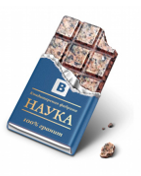
\includegraphics[width=0.8\textwidth]{image.png}
				\end{flushright}
			\end{column}
		\end{columns}
		\vspace{1.5cm}
		{\large \textbf{Лекции №1. Мера количества информации по Шеннону}}
	\end{frame}
	
	\myheadline{Определение термина \guillemotleft Информатика\guillemotright}
	\begin{frame}
		\textcolor{ForestGreen}{Информатика} - дисциплина, изучающая свойства и структуру информации, закономерности её создания, преобразования, накопления, передачи и использования.
		\newline \textcolor{ForestGreen}{Англ}: informatics = information technology + computer science + information theory
		\vspace{0.2cm}
		\begin{center}
			\textbf{Важные даты}
		\end{center}
		\begin{itemize}
			\item 1956 - появление термина \guillemotleft информатика\guillemotright (нем. Informatik, Штейнбух)
			\item 1968 - первое упоминание в СССР (информология, Харкевич)
			\item 197X - информатика стала отдельной наукой
			\item 4 декабря - день российской информатики
		\end{itemize}
	\end{frame}
	
	\myheadline{Терминология: информация и данные}
	\begin{frame}
		Международный стандарт ISO/IEC 2382:2015 
		\newline 
		«Information technology – Vocabulary» (вольный пересказ):
		
		\begin{flushright}
			\begin{minipage}{0.9\textwidth}
				\textcolor{ForestGreen}{Информация} – знания относительно фактов, событий, вещей, идей и понятий.
				
				\textcolor{ForestGreen}{Данные} – форма представления информации в виде, пригодном для передачи или обработки.
			\end{minipage}
		\end{flushright}
		
		\vspace{0.2cm}
		\color{black}$\bullet$ Что есть предмет информатики: информация или данные?
		
		%\newline
		\color{black}$\bullet$ Как измерить информацию? Как измерить данные?
		\newline
		Пример: \guillemotleft Байкал -- самое глубокое озеро Земли\guillemotright.
	\end{frame}
	
	\myheadline{Терминология: информация и данные (2)}
	\begin{frame}
		\begin{center}
			\raisebox{-0.5\height}{\fbox{\parbox{2cm}{\centering\textbf{Интуиция}}}}
			
			\raisebox{-0.4\height}{\fbox{\parbox{4cm}{\centering\textbf{Знания}}}}
			
			\raisebox{-0.5\height}{\fbox{\parbox{6cm}{\centering\textbf{Информация}}}}
			
			\raisebox{-0.5\height}{\fbox{\parbox{8cm}{\centering\textbf{Данные}}}}
			
			\raisebox{-0.5\height}{\fbox{\parbox{10cm}{\centering\textbf{Факты}}}}
		\end{center}
	\end{frame}
	
	\myheadline{Измерение количества информации}
	\begin{frame}
		\textcolor{ForestGreen}{Количество информации ≡ информационная энтропия} – это численная мера непредсказуемости информации. Количество информации в некотором объекте определяется непредсказуемостью состояния, в котором находится этот объект. 
		\vspace{0.2cm}
		
		Пусть i (s) — функция для измерения количеств информации в объекте s, состоящем из n независимых частей $s_k$, где k изменяется от 1 до n. Тогда \textcolor{ForestGreen}{свойства меры количества информации} \textbf{i(s)} таковы:
		\begin{itemize}
			\item Неотрицательность: i(s) ≥ 0.
			\item Принцип предопределённости: если об объекте уже все известно, то i(s) = 0.
			\item Аддитивность:  i(s) = $\sum_{}^{} i(s_k)$ по всем k.
			\item Монотонность: i(s) монотонна при монотонном изменении вероятностей.
		\end{itemize}
	\end{frame}
	
	\myheadline{Что такое вероятность события}
	\begin{frame}
		\begin{itemize}
			\item \textcolor{ForestGreen}{Классическое определение} (существует только равновозможных исходов эксперимента, из них m исходов приведут к событию А)
			\begin{flushright}
				\begin{minipage}{0.9\textwidth}
					{\Large $p(A) = \frac{m}{n}$}
				\end{minipage}
			\end{flushright}
			
			\item \textcolor{ForestGreen}{Статистическое определение} (в результате проведённых n экспериментов 
			события А возникло m раз)
			
			\begin{flushright}
				\begin{minipage}{0.9\textwidth}
					{\Large $p(A) = \lim_{n\to\infty}\frac{m}{n}$}
				\end{minipage}
			\end{flushright}
			
			\item \textcolor{ForestGreen}{Свойства вероятности}
			\begin{flushright}
				\begin{minipage}{0.9\textwidth}
					$0 \leq p(A) \leq 1$, 
				\end{minipage}
			\end{flushright}
			сумма вероятностей всех возможных несовместных событий равна 1
			 
		\end{itemize}
	\end{frame}
	
\end{document}